% Chapter 4 skeleton, 4.1 Carry (RQ1), 12 Oct. What the thesis plan (docs/thesis_plan_2026-10-11.md, section 4.1)
% still needs here. Fold into res_carry.tex / res_steady.tex, then delete this file and its \input.
% Run ids stay in comments; the text uses the K labels (carry), mapped in docs/figures/PROVENANCE.md.

\skel{Section 4.1 (plan 3.5 pp). The claim: one affine thrust map fits all four airframes and holds free hover
within 4\,cm without an integrator (Figure~\ref{fig:thrust_map}, exists); feeding the trackers the measured rod pull
together with the 60$^\circ$ plan took the circle from 8.25 to 2.91\,cm and the figure-eight (0.25\,m/s) from 8.2 to
3.0\,cm. Still needed: the 60$^\circ$ planned-pull circle (the falsifier, flown 14 Oct), one repeat of the measured
circle, a hover of at least 30\,s (the 3-min hover, 14 Oct). Table~\ref{tab:rig_oct7} becomes T7 with the columns
below; the steady-error table becomes T7b (source, signature, remedy). Answer RQ1 in four sentences.}

% T7: Table rig_oct7 (res_carry.tex) grows into this; the rows below are the cells still to come.
\begin{table}[htbp]
  \centering
  \footnotesize
  \caption{Carry on the rig (T7, to merge into Table~\ref{tab:rig_oct7}): the pull source and the rod plan against
  the path error. [To fill from the 14 Oct flights.]}
  \label{tab:T7}
  \begin{tabularx}{\textwidth}{lYccYccc}
    \toprule
    Flight & Path & Pull source & Rod plan & Error mean / max (cm) & Lag (s) & Height sd (cm) & $n$ \\
    \midrule
    K1 & circle 0.125\,m/s & planned & 45$^\circ$ & 8.25 / [\dots] & 0.45 & 4.8 & 1 \\ % r006
    K2 & circle 0.125\,m/s & measured & 60$^\circ$ & 2.91 / [\dots] & 0.20 & 0.5 & 1 \\ % r206e60
    K3 & circle 0.125\,m/s & measured & 60$^\circ$ & [\dots] & [\dots] & [\dots] & [\dots] \\ % 14 Oct R2 (repeat)
    K4 & circle 0.125\,m/s & planned & 60$^\circ$ & [\dots] & [\dots] & [\dots] & [\dots] \\ % 14 Oct R3 (falsifier)
    K5 & figure-eight 0.25\,m/s & planned & 45$^\circ$ & 8.2 / [\dots] & 0.41 & 4.7 & 1 \\ % r0007
    K6 & figure-eight 0.25\,m/s & measured & 60$^\circ$ & 3.0 / [\dots] & 0.21 & 0.6 & 1 \\ % r2008e60
    K7 & hover 3 min & measured & 60$^\circ$ & [\dots] & -- & [\dots] & 1 \\ % 14 Oct R1
    \bottomrule
  \end{tabularx}
\end{table}

\paragraph{The 60$^\circ$ planned-pull circle.} [Frozen falsifier, to score after 14 Oct: if K4 lies within
max(1\,cm, the lap-to-lap sd) of 2.91\,cm, the gain came from the rod angle, not the measurement.]

% 12 Oct: the figure from branch thesis-figs (docs/figures/F_rig_carry/caption.md) replaces the placeholder.
\begin{figure}[htbp]
\centering
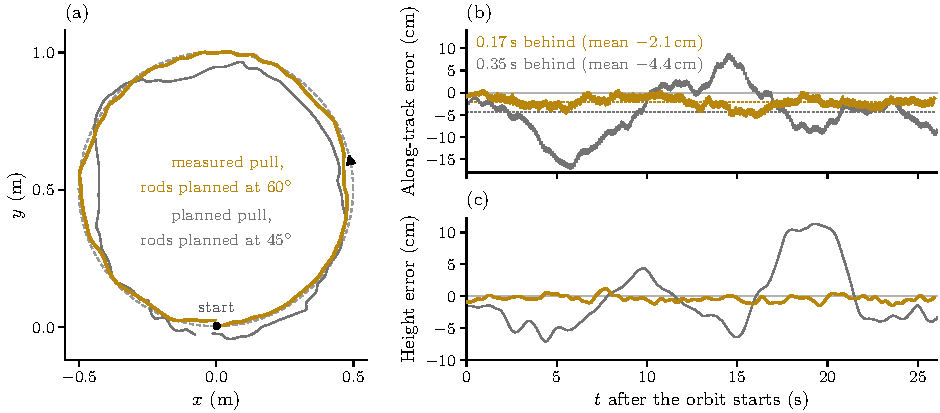
\includegraphics[width=\textwidth]{Images/rig_carry.pdf}
\caption[The circle on the rig: measured pull against planned pull]{The four-UAV circle on the rig, radius 0.5\,m at
0.125\,m/s, one lap: the trackers fed the rod pull they measure from motion capture with the rods planned at
60$^\circ$ (gold), against the same circle flown that morning on the planner's pull with the rods planned at
45$^\circ$ (grey); one run each. (a) Plan view of the ring's centre against the reference circle (dotted), with the
start and the direction of travel. (b) Along-track error, the ring's position along the circle minus the
reference's, negative behind; dotted: each run's mean, 2.1\,cm (0.17\,s) and 4.4\,cm (0.35\,s) behind, with the
worst 5.5 and 17\,cm. (c) Height error, measured minus planned, with a standard deviation of 0.5\,cm against
5.0\,cm.}
\label{fig:F8}
\end{figure}

\paragraph{Answer to RQ1.} [Four sentences: the thrust map, free hover, the measured pull with the 60$^\circ$ plan,
and what the planned-pull circle showed.]
